\documentclass[conference]{IEEEtran}
\IEEEoverridecommandlockouts

\usepackage{cite}
\usepackage{amsmath,amssymb,amsfonts}
\usepackage{graphicx}
\usepackage{textcomp}
\usepackage{xcolor}
\usepackage{booktabs}
\usepackage{multirow}
\usepackage{microtype}
\usepackage{url}
\usepackage{array}
\usepackage{tabularx}
\usepackage{pifont}
\usepackage{makecell}
\usepackage{colortbl}
\usepackage[hidelinks]{hyperref}

\newcommand{\yes}{\ding{51}}
\newcommand{\no}{\ding{55}}
\newcommand{\partly}{$\circ$}

\renewcommand{\topfraction}{0.9}
\renewcommand{\dbltopfraction}{0.9}
\renewcommand{\bottomfraction}{0.8}
\renewcommand{\textfraction}{0.07}
\renewcommand{\floatpagefraction}{0.8}
\renewcommand{\dblfloatpagefraction}{0.8}
\setcounter{topnumber}{3}
\setcounter{dbltopnumber}{3}
\setcounter{totalnumber}{4}

\title{Privacy-Preserving Federated Synthetic Data Generation for Intrusion Detection in MQTT-Based IoT Gateways}

\makeatletter
\newcommand{\linebreakand}{%
  \end{@IEEEauthorhalign}
  \hfill\mbox{}\par
  \mbox{}\hfill\begin{@IEEEauthorhalign}
}
\makeatother

\author{
\IEEEauthorblockN{Nam-Khanh Nguyen}
\IEEEauthorblockA{\textit{Faculty of Information Assurance} \\
\textit{FPT University}\\
Hanoi, Vietnam \\
southkhanh@gmail.com}
\and
\IEEEauthorblockN{Son-Truong-Giang Nguyen}
\IEEEauthorblockA{\textit{Faculty of Information Assurance} \\
\textit{FPT University}\\
Hanoi, Vietnam \\
giangnsthe190021@gmail.com}
\and
\IEEEauthorblockN{Tri-Dung Nguyen}
\IEEEauthorblockA{\textit{Faculty of Information Assurance} \\
\textit{FPT University}\\
Hanoi, Vietnam \\
dungtn002@gmail.com}
\linebreakand
\IEEEauthorblockN{Duc-Lam Vu}
\IEEEauthorblockA{\textit{Faculty of Information Assurance} \\
\textit{FPT University}\\
Hanoi, Vietnam \\
lamvdhe180242@fpt.edu.vn}
\and
\IEEEauthorblockN{Trong-Hoang-Dat Nguyen}
\IEEEauthorblockA{\textit{Faculty of Information Assurance} \\
\textit{FPT University}\\
Hanoi, Vietnam \\
endi011005@gmail.com}
\linebreakand
\IEEEauthorblockN{Anh-Nhat Nguyen}
\IEEEauthorblockA{\textit{Faculty of Information Assurance} \\
\textit{FPT University}\\
Hanoi, Vietnam \\
nhatna3@fe.edu.vn}
\and
\IEEEauthorblockN{Thanh-Tuan Nguyen}
\IEEEauthorblockA{\textit{Faculty of Information Assurance} \\
\textit{FPT University}\\
Hanoi, Vietnam \\
tuannt84@fe.edu.vn 
}
\and
\IEEEauthorblockN{Minh-Tri Luu}
\IEEEauthorblockA{\textit{Faculty of Information Assurance} \\
\textit{FPT University}\\
Hanoi, Vietnam \\
trilm29@fe.edu.vn}
}

\begin{document}

\maketitle

\begin{abstract}
Federated learning lets Internet of Things (IoT) gateways train an intrusion detection system (IDS) without pooling raw traffic, but rare attack classes are scattered across gateways and model updates can still leak training records. This paper presents PP-FedData, which adapts marginal-based private synthesis to IoT gateways. Its generator, FedDP-Marginal, releases noisy count tables in three rounds, splits integer Skellam noise across the gateways, sums the tables with the SecAgg+ secure aggregation protocol of Flower, and samples class-conditional packets from a Chow--Liu tree. A federated conditional variational autoencoder (CVAE) trained with differentially private stochastic gradient descent is the deep baseline under identical partitions, budgets and evaluation. On the DoS/DDoS-MQTT-IoT dataset, an IDS trained only on FedDP-Marginal data reaches a test macro-F1 of 0.366--0.433 at $\varepsilon = 1$--10 ($\delta = 10^{-5}$) with noise shared across honest gateways, against 0.176--0.275 for the CVAE, which adds its noise at each gateway; under that same trust model, FedDP-Marginal still leads at every budget (0.267--0.406). It transmits 0.48--0.53\,MB per run instead of 13.6--72.4\,MB, and secure aggregation costs $1.39\times$ the bytes and no utility. Synthetic data do not improve an IDS when real data can be pooled; their value lies where raw traffic must stay local. A requirement-driven rule maps trust, privacy and bandwidth requirements to a configuration.
\end{abstract}

\begin{IEEEkeywords}
Federated learning, differential privacy, secure aggregation, synthetic data, marginal-based synthesis, intrusion detection, MQTT, Internet of Things.
\end{IEEEkeywords}

\section{Introduction}\label{sec:intro}

The Message Queuing Telemetry Transport (MQTT) protocol carries the publish-subscribe traffic of many Internet of Things (IoT) deployments, and its brokers are exposed to denial-of-service (DoS) and distributed DoS (DDoS) attacks that abuse the protocol itself. The DoS/DDoS-MQTT-IoT dataset, captured on a physical testbed, records normal MQTT traffic together with ten such attack scenarios~\cite{alatram2023}. Intrusion detection systems (IDSs) based on machine learning learn these attacks from labeled traffic, which in practice is spread over gateways that cannot pool it. Federated learning (FL) trains a shared model while the data stay local: a server aggregates the clients' updates over several rounds, for example by federated averaging (FedAvg)~\cite{mcmahan2017}; here the clients are the gateways. Keeping data local does not remove the privacy risk, because shared gradients can reveal training records~\cite{zhu2019}, and privacy-preserving FL for IoT intrusion detection remains an active field~\cite{vyas2024}.

Two difficulties combine in this setting. First, rare attack classes are scattered unevenly across gateways, so the data are not independent and identically distributed (non-IID): a gateway may hold a handful of packets of a rare attack, or none. Second, the two standard protections answer different threats. Secure aggregation (SecAgg) and its scalable variant SecAgg$^+$ hide each client's update from the server and reveal only their sum~\cite{bonawitz2017, bell2020}, but say nothing about what the sum, the model or its synthetic data reveal. Differential privacy (DP) bounds that disclosure for any single record~\cite{dwork2014}, at a cost in utility. Generative models, reviewed in~\cite{deng2025}, have been trained federatedly to synthesize the missing attack traffic~\cite{hamouda2024, yao2024, shettar2026}. They exchange full models over many rounds and, when trained with DP stochastic gradient descent (DP-SGD)~\cite{abadi2016dpsgd}, spread the privacy noise over thousands of optimization steps.

Marginal-based synthesis instead measures low-order count tables with DP noise and samples records from a graphical model fitted to them~\cite{zhang2017privbayes, mckenna2021mst, mckenna2024aim}. Count tables are sums over records, which is exactly what secure aggregation computes, so discrete noise such as the Skellam distribution can be split across gateways and the server sees only the noisy sum~\cite{kairouz2021, agarwal2021}. Federated marginal synthesizers exist~\cite{maddock2024, pentyala2024} and have been evaluated on general tabular benchmarks; neither their downstream detection of rare attacks in IoT traffic nor a comparison with a federated deep generator under the same protections has been measured.

This paper studies that comparison on MQTT traffic with PP-FedData, a privacy-preserving federated data generation framework, through four research questions:
\begin{itemize}
    \item RQ1: How much IDS utility does federated synthetic data retain when raw traffic cannot be pooled, and does it add utility when real data are available?
    \item RQ2: Under the same $(\varepsilon, \delta)$ budget, how does a federated marginal generator compare with a federated conditional variational autoencoder (CVAE) trained with DP-SGD in utility, rare-class recall and communication?
    \item RQ3: What does each protection (DP, SecAgg$^+$, both) cost and protect, as a function of the protected unit (packet, TCP stream, capture) and of the number of honest gateways?
    \item RQ4: Which configuration should a deployment choose given its trust, privacy and bandwidth requirements?
\end{itemize}

We do not claim a new synthesis algorithm: FedDP-Marginal adapts tree-structured marginal synthesis~\cite{chow1968, mckenna2021mst}, and federated marginal synthesis has been studied before~\cite{maddock2024, pentyala2024}. Our contribution lies in combining these components for IoT gateways and in a controlled empirical comparison:
\begin{enumerate}
    \item FedDP-Marginal is a three-release protocol for IoT-MQTT traffic in which gateways add shares of integer Skellam noise to their count tables and sum them with the SecAgg$^+$ implementation of the Flower framework; the privacy loss is accounted exactly and reported for every number of honest gateways, with options for a threshold of honest gateways, client-side DP, and stream- or capture-level protection.
    \item A controlled benchmark compares it with a federated CVAE on the same non-IID partitions, privacy budgets, secure aggregation and evaluation, and separates the cost of DP, the cost of SecAgg$^+$ and the effect of the generator family.
    \item A requirement-driven configuration guide filters the measured configurations by trust, privacy budget, bandwidth and attack priority and selects from their Pareto front.
\end{enumerate}

Section~\ref{sec:related_work} reviews related work, Section~\ref{sec:methodology} describes the system model and the two generators, Section~\ref{sec:setup} gives the experimental setup, Section~\ref{sec:results} reports and discusses the results, and Section~\ref{sec:conclusion} concludes.

\section{Related Work}\label{sec:related_work}

\subsection{Privacy Protection in Federated Learning}
A survey of privacy-preserving FL for IoT intrusion detection groups the techniques into differential privacy, homomorphic encryption, secure multi-party computation (MPC), trusted execution environments and blockchain~\cite{vyas2024}. The last three require heavy computation, special hardware or consensus overhead on constrained gateways, so this work uses DP and secure aggregation.

\textit{Differential privacy} limits how much a released output can change when one record is added or removed~\cite{dwork2014}. In the central model a trusted curator adds the noise; in the classical local model every individual record is randomized before it leaves its owner, at a much higher noise level. Between the two, this paper uses \textit{client-side DP}: each gateway adds enough noise for its own release to satisfy DP by itself, so it needs to trust neither the server nor the other gateways. DP-SGD clips per-example gradients and adds Gaussian noise at every step~\cite{abadi2016dpsgd}; its cumulative loss is tracked with R\'enyi DP (RDP)~\cite{mironov2017rdp}.

\textit{Secure aggregation} lets the server learn only the sum of client vectors. The protocol of Bonawitz \textit{et~al.}\ uses pairwise masks and secret sharing to tolerate dropouts~\cite{bonawitz2017}; SecAgg$^+$ replaces the complete communication graph with a sparse random graph and reaches polylogarithmic overhead~\cite{bell2020}. Secure aggregation adds no statistical noise, but it protects only the individual updates, not the aggregate.

\textit{Distributed DP} combines both: each client adds a share of the noise and secure aggregation reveals only the sum, which then carries the full calibrated noise. Because secure aggregation works on integers modulo $2^b$, discrete mechanisms are needed. Kairouz \textit{et~al.}\ proposed the distributed discrete Gaussian~\cite{kairouz2021}. Agarwal \textit{et~al.}\ showed that the Skellam distribution is closed under summation and gave a tight RDP bound for it~\cite{agarwal2021}. Both apply it to multi-round FL training, adding the noise once per round to the securely summed client updates; count tables, each a single sum, are a particularly simple fit.

\subsection{Synthetic Data for Intrusion Detection}
Oversampling such as the synthetic minority oversampling technique (SMOTE) interpolates between minority neighbors~\cite{chawla2002}, which requires the minority records to be pooled and is therefore unavailable when a gateway holds few or no attack records. A systematic review of generative AI for IoT intrusion detection found that most studies use generative adversarial networks (GANs) or variational autoencoders for augmentation and class rebalancing, with mode collapse and training instability as recurring problems~\cite{deng2025}. Hamouda \textit{et~al.}\ trained a federated conditional GAN on Edge-IIoTset and applied DP-SGD only to the downstream classifier; they identified cryptographic protection of the models as an open challenge~\cite{hamouda2024}. Yao \textit{et~al.}\ protected the downlink broadcast of synthetic samples with dynamic $(t, n)$-threshold secret sharing, while the uplink gradients relied on Gaussian DP~\cite{yao2024}. Shettar \textit{et~al.}\ reported a detection F1-score of 96.8\% with a central aggregator under DP at $\varepsilon = 4.8$~\cite{shettar2026}. None of these works applies secure aggregation to the generator updates or measures how DP and secure aggregation each affect rare-class detection.

\subsection{Marginal-Based Private Synthesis}
Marginal-based synthesizers avoid backpropagation altogether. PrivBayes fits a Bayesian network to noisy low-order marginals~\cite{zhang2017privbayes}; MST measures noisy two-way marginals along a maximum spanning tree and post-processes them with a graphical model~\cite{mckenna2021mst}; AIM selects marginals adaptively and iteratively~\cite{mckenna2024aim}. Two works move this family to distributed data. FLAIM adapts AIM to federated clients under zero-concentrated DP and compares it with a secure multi-party variant~\cite{maddock2024}. CaPS performs marginal selection and measurement inside secure multi-party computation (``DP-in-MPC'')~\cite{pentyala2024}. Both were evaluated mainly on general-purpose tabular benchmarks; FLAIM also used the legacy DARPA intrusion detection data and measured workload error and negative log-likelihood, not downstream rare-class detection. The family models only low-order dependencies, must discretize continuous attributes, and has a low signal-to-noise ratio in sparse cells.

\subsection{Research Gap}
Table~\ref{tab:lit_review} summarizes the closest works. Based on a non-systematic search of the literature, and to the best of our knowledge, no prior study (i) evaluates a federated marginal generator on IoT-MQTT traffic for downstream rare-class detection, (ii) compares it with a federated deep generator under identical partitions, budgets and secure aggregation, or (iii) combines distributed discrete DP with a working secure aggregation implementation and reports the guarantee as a function of the number of honest clients.

\begin{table}[!t]
\centering
\caption{Comparison With the Closest Related Work}
\label{tab:lit_review}
\scriptsize
\setlength{\tabcolsep}{3.2pt}
\begin{tabular}{l c c c c c c c c}
\toprule
\textbf{Work} & \textbf{FL} & \textbf{IoT} & \textbf{Syn.} & \textbf{DP} & \textbf{SA} & \textbf{Marg.} & \textbf{D-DP} & \textbf{IDS} \\
\midrule
Hamouda \textit{et al.}~\cite{hamouda2024}  & \yes & \yes & \yes & \partly & \no  & \no  & \no  & \yes \\
Yao \textit{et al.}~\cite{yao2024}          & \yes & \yes & \yes & \yes & \partly & \no  & \no  & \yes \\
Shettar \textit{et al.}~\cite{shettar2026}  & \yes & \yes & \yes & \yes & \no  & \no  & \no  & \yes \\
Kairouz \textit{et al.}~\cite{kairouz2021}  & \yes & \no  & \no  & \yes & \yes & \no  & \yes & \no  \\
Agarwal \textit{et al.}~\cite{agarwal2021}  & \yes & \no  & \no  & \yes & \yes & \no  & \yes & \no  \\
MST~\cite{mckenna2021mst}          & \no  & \no  & \yes & \yes & \no  & \yes & \no  & \no  \\
FLAIM~\cite{maddock2024}           & \yes & \no  & \yes & \yes & \yes & \yes & \no  & \no  \\
CaPS~\cite{pentyala2024}           & \no  & \no  & \yes & \yes & \yes & \yes & \no  & \no  \\
\rowcolor{gray!15}
PP-FedData                         & \yes & \yes & \yes & \yes & \yes & \yes & \yes & \yes \\
\bottomrule
\end{tabular}

\vspace{2pt}
\parbox{\columnwidth}{\scriptsize Syn.: synthetic data generation; SA: secure aggregation or MPC; Marg.: marginal-based DP synthesis; D-DP: distributed DP; IDS: downstream intrusion detection evaluated. \partly: partly addressed (Hamouda \textit{et al.}\ apply DP to the classifier, not the generator; Yao \textit{et al.}\ use secret sharing on the downlink only).}
\end{table}

\section{System Model and Methodology}\label{sec:methodology}

\subsection{Architecture and Threat Model}\label{subsec:system}
Fig.~\ref{fig:architecture} shows the three parties of PP-FedData. A federation of $K$ edge gateways $\mathcal{K} = \{1, \dots, K\}$ observes MQTT traffic; gateway $k$ keeps its packets $\mathcal{D}_k$ locally. An aggregation server coordinates the rounds, reconstructs a global generator from the aggregated releases and samples synthetic packets for every class. A downstream IDS is trained on the synthetic packets, alone or with real ones, and is evaluated on real traffic. Two generator routes share this architecture: FedDP-Marginal, which exchanges count tables in three releases, and a federated CVAE, which exchanges model weights over tens of FedAvg rounds.

To model non-IID gateways, the training data are partitioned with the label-skew scheme of Hsu \textit{et~al.}~\cite{hsu2019}: for each class $c \in \{1, \dots, C\}$ the shares of the $K$ gateways are drawn as
\begin{equation}
\mathbf{p}_c = (p_{c,1}, \dots, p_{c,K}) \sim \mathrm{Dir}(\alpha_{\mathrm{dir}} \mathbf{1}_K),
\label{eq:dirichlet}
\end{equation}
and each record of class $c$ goes to gateway $k$ with probability $p_{c,k}$. With $K = 5$ and $\alpha_{\mathrm{dir}} = 0.5$, some gateways receive few or no packets of a rare attack class.

\textit{Threat model.} The server is honest-but-curious: it follows the protocol but inspects everything it receives. Gateways follow the protocol; poisoning and Byzantine behavior are out of scope. The two protections answer different threats. SecAgg$^+$~\cite{bell2020} hides each gateway's contribution from the server, which learns only the sum. DP bounds what the released sum, and every model or synthetic record derived from it, reveals about one record~\cite{dwork2014}. By default the protected record is one packet; Section~\ref{subsec:accounting} extends the unit to a TCP stream or a capture. Class labels, class quotas, the gateways' sample counts and the preprocessing statistics are treated as public side information outside $\varepsilon$.

\begin{figure*}[!t]
\centering
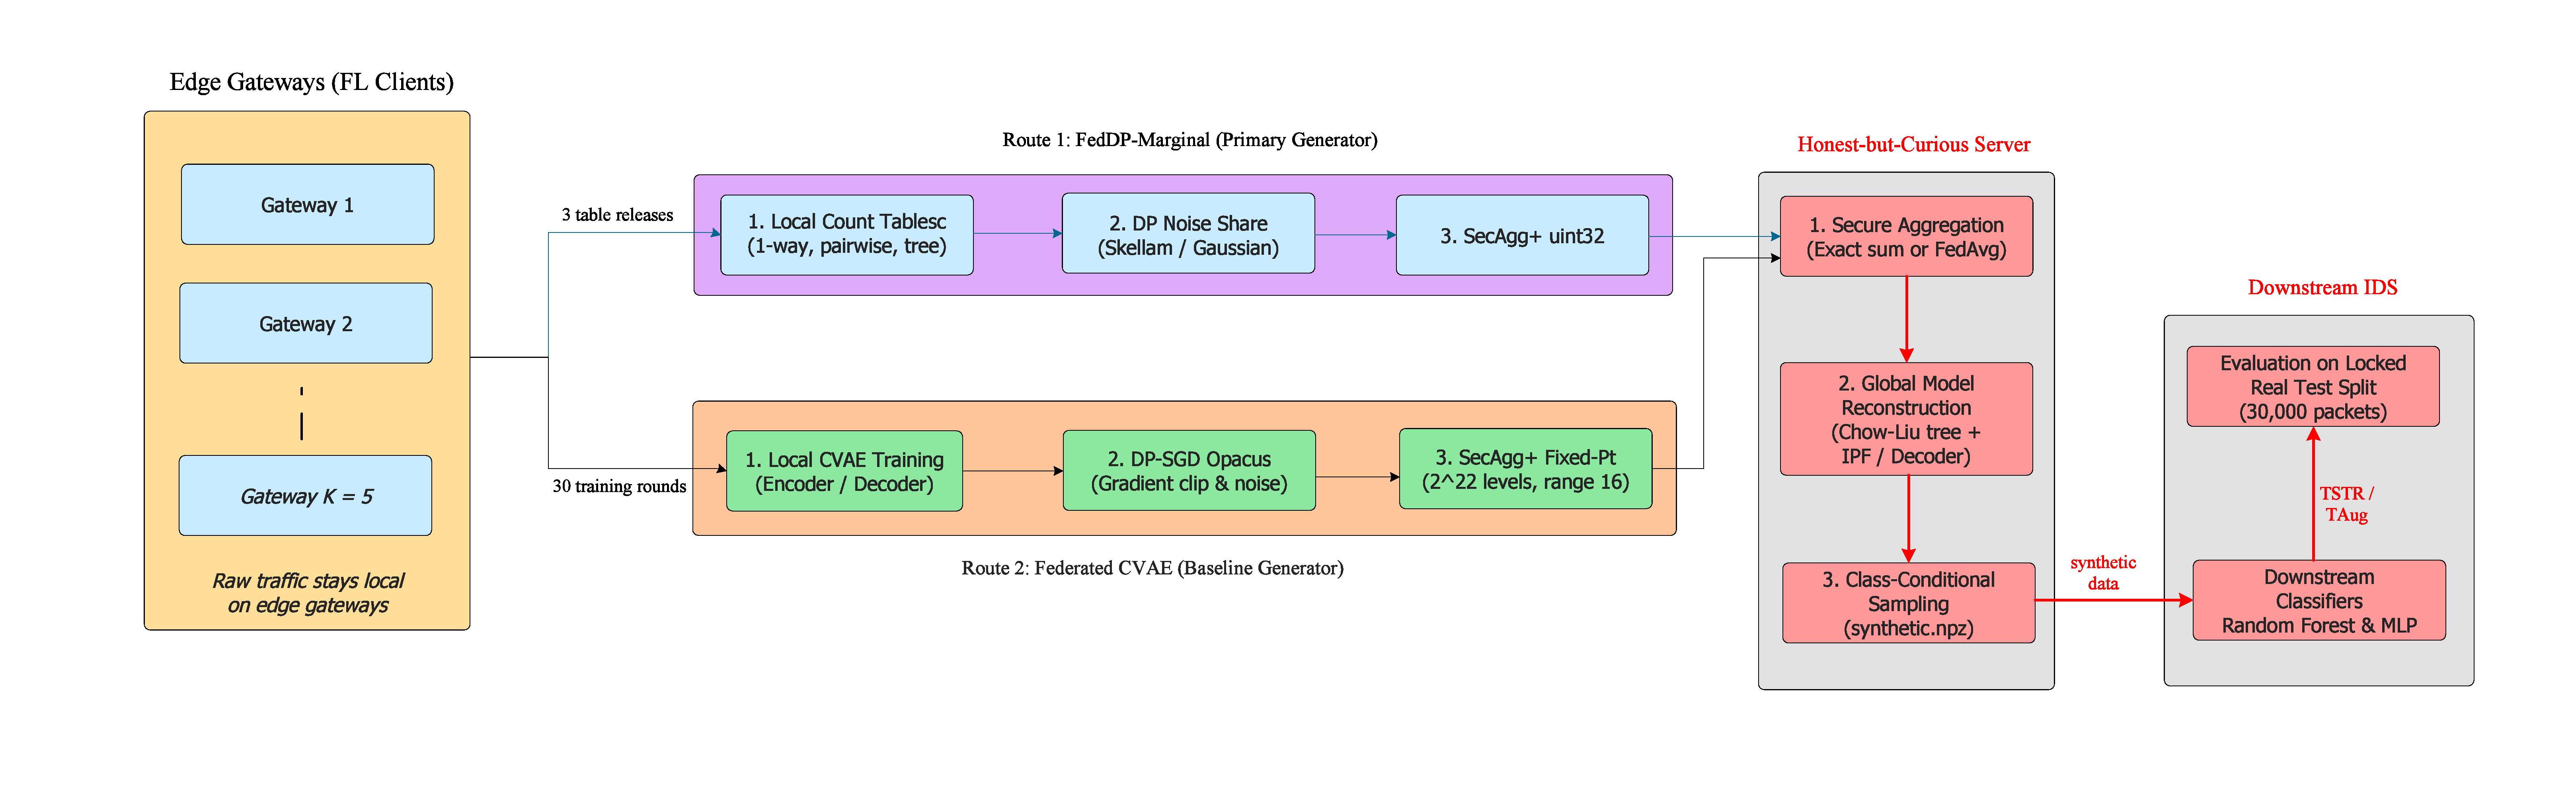
\includegraphics[width=\textwidth]{graphics/paper/fig1_architecture.pdf}
\caption{PP-FedData architecture. Gateways keep raw traffic; FedDP-Marginal sends three releases of noisy count tables and the federated CVAE sends model updates, both through SecAgg$^+$ to an honest-but-curious server, which samples synthetic packets for the downstream IDS.}
\label{fig:architecture}
\end{figure*}

\subsection{FedDP-Marginal}\label{subsec:feddp_marginal}
FedDP-Marginal adapts tree-structured marginal synthesis~\cite{chow1968, mckenna2021mst} to a federation. It models $d = 37$ attributes: 13 numeric attributes, discretized into $B_{\mathrm{fine}} = 64$ equal bins on the standardized range $[-5, 5]$; 19 binary attributes (7 protocol flags and 12 missingness indicators); and 5 categorical attributes (message type, two quality-of-service (QoS) fields, requested QoS and protocol). Every table is a sum over records, so each release is a single additive query. The protocol has three releases (Fig.~\ref{fig:three_release}):
\begin{enumerate}
    \item In Release~1, each gateway counts every attribute per class on fine bins. From the noisy sum the server places $B_{\mathrm{coarse}}$ coarse bins at the quantiles of each numeric attribute and broadcasts the cut points.
    \item In Release~2, gateways count all $\binom{37}{2} = 666$ attribute pairs on coarse values, pooled over classes. The server estimates the mutual information $\hat{I}$ of every pair from the noisy tables (counts clipped at zero and smoothed) and builds a single Chow--Liu tree~\cite{chow1968}:
    \begin{equation}
    T^\star = \arg\max_{T} \sum_{(i,j) \in T} \hat{I}(X_i; X_j),
    \label{eq:chow_liu}
    \end{equation}
    with $\hat{I}(X_i; X_j) = \sum_{a,b} \hat{p}(a,b) \log \frac{\hat{p}(a,b)}{\hat{p}(a)\hat{p}(b)}$, and broadcasts $T^\star$.
    \item In Release~3, gateways count the $(\mathrm{root}, y)$ table and the $(\mathrm{parent}, \mathrm{child}, y)$ table of every tree edge on coarse values.
\end{enumerate}
Pooling Release~2 over classes is deliberate: a per-class split would divide the signal of each cell by about $C$ while the sensitivity stays the same, which corrupts the tree. Class-specific structure enters through Release~3.

\textit{Sampling.} For each class $c$ the server samples records along $T^\star$ from the root to the leaves (conditioning on $y = c$ is written as $c$),
\begin{equation}
\hat{P}(\mathbf{x} \mid c) = \hat{P}(x_r \mid c) \prod_{(u,v) \in T^\star} \hat{P}(x_v \mid x_u, c),
\label{eq:tree_factorization}
\end{equation}
where $r$ is the root attribute and every edge $(u,v)$ of $T^\star$ is oriented away from $r$, so that $u$ is the parent of $v$. A sampled coarse value of a numeric attribute is refined to a fine bin with the class's fine histogram from Release~1 and then drawn uniformly inside it. The records are mapped back to the feature space by inverting the preprocessing.

\textit{Post-processing (MGr).} The refined variant combines every independent noisy estimate of an attribute's class-conditional marginal (from Release~1 and from the incident tree tables) by inverse-variance weighting, clips negative counts, adjusts each edge table to the fused marginals with iterative proportional fitting, and may re-root the tree at the attribute with the largest total noisy mutual information. Because it only transforms released values, it costs no privacy budget~\cite{dwork2014}.

\begin{figure*}[!t]
\centering
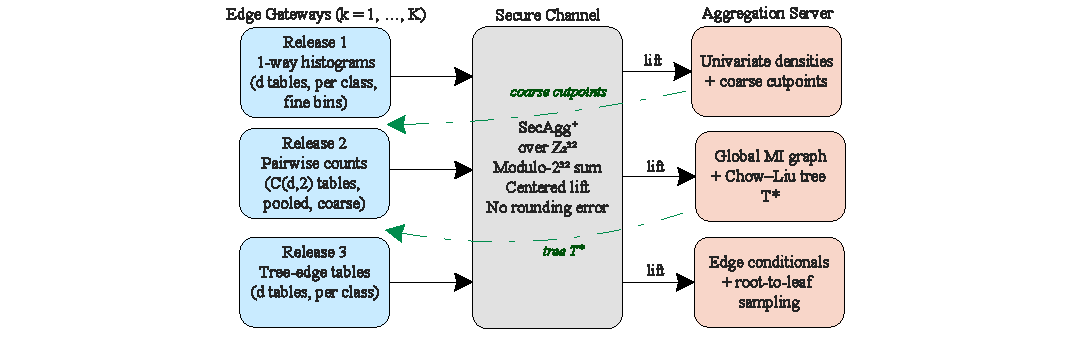
\includegraphics[width=\textwidth]{graphics/paper/Fig2.pdf}
\caption{Three-release protocol of FedDP-Marginal. Each release is a sum of count tables plus Skellam noise shares, computed with SecAgg$^+$ over $\mathbb{Z}_{2^{32}}$. The coarse cut points (after Release~1) and the tree $T^\star$ (after Release~2) are broadcast back before the next release.}
\label{fig:three_release}
\end{figure*}

\subsection{Privacy Accounting}\label{subsec:accounting}
\textit{Sensitivity.} Two datasets are neighbors if they differ by one packet. A packet adds one count to one cell of every table it touches, so a release of $M_r$ tables (37, 666 and 37 for the three releases) has $\ell_1$ and $\ell_2$ sensitivities $\Delta_{1,r} = M_r$ and $\Delta_{2,r} = \sqrt{M_r}$. To protect a unit of several packets (a TCP stream or a capture), each unit is assigned to a single gateway, which uses at most $m$ of its packets. The sensitivities then become
\begin{equation}
\Delta_{1,r} = m\,M_r, \qquad \Delta_{2,r} = m\sqrt{M_r}.
\label{eq:sensitivity}
\end{equation}

\textit{Skellam mechanism.} The noise of each cell follows the Skellam distribution $\mathrm{Sk}(\mu) = \mathrm{Pois}(\mu/2) - \mathrm{Pois}(\mu/2)$, which has zero mean and variance $\mu$ and is closed under summation~\cite{agarwal2021}. Agarwal \textit{et~al.}\ write the symmetric Skellam as $\mathrm{Sk}_{\mu,\mu}$, with variance $2\mu$; \eqref{eq:skellam_rdp} is their bound rewritten in terms of the variance. For an integer order $\lambda > 1$, a release with variance $\mu_r$ per cell satisfies the RDP bound of Agarwal \textit{et~al.}~\cite[Cor.~3.6]{agarwal2021}:
\begin{equation}
\begin{aligned}
\varepsilon_r(\lambda) \le{}& \frac{\lambda \Delta_{2,r}^2}{2\mu_r} \\
&+ \min\!\left( \frac{(2\lambda - 1)\Delta_{2,r}^2 + 6\Delta_{1,r}}{4\mu_r^2}, \frac{3\Delta_{1,r}}{2\mu_r} \right).
\end{aligned}
\label{eq:skellam_rdp}
\end{equation}
RDP composes additively over the three releases~\cite{mironov2017rdp}, and the total is converted to $(\varepsilon, \delta)$-DP with the conversion used by the Opacus accountant~\cite{yousefpour2021}:
\begin{equation}
\varepsilon = \min_{\lambda} \Big[ \sum_{r=1}^{3} \varepsilon_r(\lambda) - \frac{\ln \delta + \ln \lambda}{\lambda - 1} + \ln \frac{\lambda - 1}{\lambda} \Big],
\label{eq:rdp_conversion}
\end{equation}
over $\lambda \in \{2, \dots, 63\} \cup \{64, 72, \dots, 1024\}$. The budget is split over the releases by a vector $\mathbf{s} = (s_1, s_2, s_3)$ through $\mu_r = \Delta_{2,r}^2 / (2 s_r \kappa)$, where $\kappa$ is the largest value, found by bisection, for which \eqref{eq:rdp_conversion} meets the target $\varepsilon$. The split and $B_{\mathrm{coarse}}$ are chosen on validation data from $\mathbf{s} \in \{(0.3, 0.1, 0.6), (0.5, 0.1, 0.4), (0.15, 0.05, 0.8)\}$ and $B_{\mathrm{coarse}} \in \{4, 8, 16, 32\}$; the selected settings are 16 bins with $(0.3, 0.1, 0.6)$ at $\varepsilon = 1$, 16 bins with $(0.15, 0.05, 0.8)$ at $\varepsilon = 5$, and 8 bins with $(0.5, 0.1, 0.4)$ at $\varepsilon = 10$.

\textit{Noise sharing and trust.} Gateway $k$ adds integer noise $\xi_k \sim \mathrm{Sk}(\mu_r / t)$ to every cell. With $t = K$ (the default, MGs and MGr) the full variance is reached when all gateways are honest. If only $h$ gateways add their share, the aggregate variance is $h\mu_r/t$, and the guarantee is recomputed from \eqref{eq:skellam_rdp}--\eqref{eq:rdp_conversion} and reported for every $h$. A threshold $t < K$ keeps the target $\varepsilon$ whenever at least $t$ gateways are honest, at the price of more noise when all are. In the client-side variant (MGl), every gateway adds the full variance $\mu_r$, so its own release is DP by itself and it trusts neither the server nor the other gateways; the sum then carries $K\mu_r$.

\textit{Secure transport.} The noisy integer tables are summed with Flower's SecAgg$^+$~\cite{beutel2020, bell2020} over $\mathbb{Z}_{2^{32}}$:
\begin{equation}
S = \sum_{k \in \mathcal{K}} (\mathbf{x}_k + \boldsymbol{\xi}_k) \bmod 2^{32},
\label{eq:secagg}
\end{equation}
where $\mathbf{x}_k$ are gateway $k$'s counts; the server lifts every entry $S \ge 2^{31}$ to $S - 2^{32}$ to recover negative values. Since the counts are at most $n = 88{,}500$ and the noise is small compared with $2^{31}$, the lifted sum equals the exact noisy sum: secure aggregation adds no rounding error and receives no privacy credit. Because each release is a single sum, splitting the noise across gateways is valid. The CVAE baseline instead runs record-level DP-SGD with many local steps per round, whose noise is added inside each gateway's optimization and cannot be split this way. FL training can use distributed noise when each gateway sends one clipped update per round and the noise is added to their sum (DP-FedSGD)~\cite{kairouz2021, agarwal2021}; we implemented such a CVAE variant but did not run it.

\subsection{Federated CVAE Baseline}\label{subsec:cvae}
The deep baseline is a label-conditional CVAE~\cite{sohn2015cvae} on the $p = 59$ encoded features, without batch normalization so that per-example gradients are independent. It is trained with FedAvg~\cite{mcmahan2017} for 30 rounds of 2 local epochs (B3). The DP variant (M1) runs DP-SGD with Opacus~1.6.0~\cite{abadi2016dpsgd, yousefpour2021}: per-example gradients are clipped and noised at every local step,
\begin{equation}
\tilde{g} = \frac{1}{b} \Big( \sum_{i=1}^{b} \frac{g_i}{\max(1, \|g_i\|_2 / G)} + \mathcal{N}(0, \sigma_k^2 G^2 \mathbf{I}) \Big),
\label{eq:dpsgd}
\end{equation}
where $g_i$ is the gradient of example $i$ in a minibatch of size $b$, $G$ is the clipping bound, and the noise multiplier $\sigma_k$ is calibrated for each gateway; the federation reports the worst case $\varepsilon = \max_k \varepsilon_k$. M2 aggregates the weights with SecAgg$^+$ (5 shares, reconstruction threshold 3, clipping range 16, $2^{22}$ quantization levels), and M3 combines M1 and M2. Even with SecAgg$^+$, the CVAE route provides client-side DP only. Message sizes differ because the networks do: hidden layers (256, 128) for B3 and M2, (128, 64) for M1 and M3, and widths of 64 to 128 with latent size 16 for the re-tuned M1o and M3o. Synthetic records are decoded from $z \sim \mathcal{N}(0, \mathbf{I})$; the DP configurations use the plain decoder, which depends only on the DP-trained weights, whereas the non-private B3 and M2 use a residual-noise decoder with per-class variances estimated on the pooled training data. The federated CVAE was the initial design choice; because its utility under DP stayed low even after per-$\varepsilon$ re-tuning at full federated scale (M1o, M3o), FedDP-Marginal became the main generator and the CVAE is retained as the baseline.

\section{Experimental Setup}\label{sec:setup}

\subsection{Dataset and Preprocessing}\label{subsec:dataset}
We use the DoS/DDoS-MQTT-IoT dataset~\cite{alatram2023}: 39,000,601 packets, each described by 33 columns, with normal traffic and the DoS and DDoS variants of five MQTT attack families. The attack rows are the authors' CSV exports. Normal traffic is released only as packet capture (PCAP) files, so we exported it with TShark into the same columns using the authors' export settings (two-pass dissection, packets sent to the broker), which reproduce their attack rows exactly in 47 of 48 captures. The DoS and DDoS sub-classes of each family are merged into one class, so that the IDS detects the attack family. Separating them is hard at the packet level: a random forest on real data reaches a macro-F1 of only 0.336 on the eleven sub-classes (normal traffic and ten attack sub-classes), and the two sub-classes of basic connect flooding are close to chance (0.59 for two classes). Merging gives six classes (Table~\ref{tab:data}).

Identifiers and capture metadata (frame number, absolute and relative timestamps, source address, free-text information) are removed to avoid leakage~\cite{arp2022}. Numeric features with skewness above 2 are log-transformed, all numeric features are standardized and clipped at $\pm 5\sigma$, and categorical fields are one-hot encoded, giving $p = 59$ features. The preprocessing statistics are fitted on the pooled training split, a centralized step outside $\varepsilon$ (Section~\ref{subsec:limitations}). Diagnostic checks found no shortcut feature: no single column reaches a macro-F1 above 0.9, the missingness indicators alone reach 0.18 (chance 0.17), and a random row split scores only 0.009 above a split by capture group.

Where a sub-class spans several capture groups (normal traffic has 49), whole groups are assigned to the training, validation or test split. Eight of the ten attack sub-classes come from a single capture file; as an exception, their validation and test rows are contiguous blocks of that capture, separated by 1,000-row buffers, and TCP streams crossing a block boundary are dropped. Neighboring blocks can still share temporal context, so leakage is reduced but not excluded; re-running the study with two other choices of test groups kept 8 of 10 verdicts. Rows are then sampled to fixed quotas (Table~\ref{tab:data}). The training quotas impose a 60:1 imbalance between \texttt{NORMAL} and \texttt{WILL}. The validation and test sets are class-balanced, so that the metrics are not dominated by the majority class. The test set (11 capture groups, 20,485 TCP streams) is used only once for the final evaluation. We call \texttt{DELAYED}, \texttt{SYN}, \texttt{INVALID} and \texttt{WILL} the rare classes.

\begin{table}[!t]
\centering
\caption{Classes, Raw Packet Counts and Split Quotas}
\label{tab:data}
\scriptsize
\setlength{\tabcolsep}{4pt}
\begin{tabular}{l r r r r r}
\toprule
\textbf{Class} & \textbf{Raw packets} & \textbf{Share} & \textbf{Train} & \textbf{Val.} & \textbf{Test} \\
\midrule
\texttt{NORMAL}  & 24,955,877 & 63.99\% & 60,000 & 2,000 & 5,000 \\
\texttt{BCF}     & 12,280,874 & 31.49\% & 20,000 & 2,000 & 5,000 \\
\texttt{DELAYED} &    601,542 &  1.54\% &  3,000 & 2,000 & 5,000 \\
\texttt{SYN}     &    601,439 &  1.54\% &  3,000 & 2,000 & 5,000 \\
\texttt{INVALID} &    290,340 &  0.74\% &  1,500 & 2,000 & 5,000 \\
\texttt{WILL}    &    270,529 &  0.69\% &  1,000 & 2,000 & 5,000 \\
\midrule
\textbf{Total}   & 39,000,601 & 100\%   & 88,500 & 12,000 & 30,000 \\
\bottomrule
\end{tabular}

\vspace{2pt}
\parbox{\columnwidth}{\scriptsize BCF: basic connect flooding; DELAYED: delayed connect flooding; SYN: SYN TCP flooding; INVALID: invalid subscription flooding; WILL: connect flooding with WILL payload.}
\end{table}

\subsection{Configurations}
Table~\ref{tab:configs} lists the configurations. The real-data references B0, B1a and B1b pool the raw training data and are therefore not available in a federation. All federated configurations use $K = 5$ gateways and the partition of \eqref{eq:dirichlet} with $\alpha_{\mathrm{dir}} = 0.5$, drawn once per seed and shared by every configuration. Privacy budgets are $\varepsilon \in \{1, 5, 10\}$ with $\delta = 10^{-5}$ at the packet level; this $\delta$ is below $1/n \approx 1.13 \times 10^{-5}$ for the $n = 88{,}500$ training packets, but not far below it. The headline FedDP-Marginal configurations are MG-eps1 = MGs-eps1, MG-eps5 = MGr-eps5 and MG-eps10 = MGs-eps10, the variants selected on validation data. Hyperparameters were tuned on the validation split only (tree-structured Parzen search for the CVAE, a grid for FedDP-Marginal); this selection is not covered by $\varepsilon$.

\begin{table}[!t]
\centering
\caption{Evaluated Configurations}
\label{tab:configs}
\scriptsize
\setlength{\tabcolsep}{3pt}
\begin{tabularx}{\columnwidth}{l l >{\raggedright\arraybackslash}X c}
\toprule
\textbf{ID} & \textbf{Generator} & \textbf{Protection} & \textbf{Rounds} \\
\midrule
B0, B1a, B1b & none & pooled real data; B1a class weights, B1b SMOTE~\cite{chawla2002} & -- \\
B3           & CVAE & none (FedAvg) & 30 \\
M1-eps\{1,5,10\} & CVAE & DP-SGD at each gateway (client-side DP) & 30 \\
M2           & CVAE & SecAgg$^+$ & 30 \\
M3-eps5      & CVAE & DP-SGD and SecAgg$^+$ & 30 \\
M1o, M3o     & CVAE & as M1, M3, re-tuned per $\varepsilon$ at full scale & 15--50 \\
MGp-nodp     & Marginal & none (plain Flower sum) & 3 \\
MGs-nodp     & Marginal & SecAgg$^+$ without noise & 3 \\
MGs-eps\{1,5,10\} & Marginal & distributed Skellam DP and SecAgg$^+$ & 3 \\
MGr-eps\{1,5,10\} & Marginal & MGs with post-processing (no extra $\varepsilon$) & 3 \\
MGl-eps\{1,5,10\} & Marginal & client-side DP, plain sum & 3 \\
FedMLP       & none & IDS trained by FL; none, SecAgg$^+$, DP-SGD or DP-FedSGD & 30, 2,593 \\
\midrule
\multicolumn{4}{p{\dimexpr\columnwidth-2\tabcolsep\relax}}{Suffixes: \texttt{-t2}, \texttt{-t3}: noise share $1/t$ (holds with $t$ honest gateways); \texttt{-strm1}, \texttt{-cap50}: protect a TCP stream or a capture with at most $m = 1$ or 50 packets each. Ablations: MGd (Gaussian noise shared across gateways, secure sum simulated in-process) and MGb (second-order Bayesian network).} \\
\bottomrule
\end{tabularx}
\end{table}

\subsection{Evaluation Protocols and Metrics}
All protocols are scored on the same real test set. \textit{Train on real, test on real} (TRTR) trains the IDS on the pooled real training data (B0, B1a, B1b). \textit{Train on synthetic, test on real} (TSTR)~\cite{esteban2017} trains it on 5,000 synthetic rows per class only, which measures what a federation obtains when raw data cannot be pooled. \textit{Training augmentation} (TAug) adds synthetic rows to the pooled real data until each class has at least 20,000 rows. \textit{Local augmentation} lets each gateway train its own IDS on its local rows, topped up with synthetic rows for every class of which it holds fewer than 5,000 rows (5 gateways $\times$ 3 seeds $= 15$ models). The IDS is a random forest (RF) with 200 trees or a multilayer perceptron (MLP) with hidden layers (128, 64); for each protocol the classifier with the higher validation macro-F1 is reported.

Utility is measured by macro-F1 over the six classes (primary metric), binary F1 (normal versus attack) and rare-class recall (mean recall of the four rare classes). Fidelity is measured by the Wasserstein-1 distance, the Jensen--Shannon divergence, a correlation distance, and a classifier two-sample test (C2ST) whose area under the ROC curve (AUC) is 0.5 when synthetic and real rows are indistinguishable~\cite{lopezpaz2017}. Privacy is assessed with the formal $\varepsilon$, recomputed independently, and with three membership inference attacks (MIAs): one on the synthetic data, one with access to the released model and calibrated with a reference model~\cite{carlini2022}, and one on the released tables of FedDP-Marginal. Each attack is checked against a positive control on which it must succeed. Communication is the payload measured on the Flower message grid, reported per round and per run.

\subsection{Decision Rule and Environment}
Every configuration is run with seeds $\{0, 1, 2\}$, which govern the partition, initialization and sampling. A configuration $A$ is declared better or worse than $B$ only if
\begin{equation}
0 \notin \mathrm{CI}_{95\%}(\bar{\Delta}) \quad \text{and} \quad |\bar{\Delta}| > \max(\mathrm{sd}_A, \mathrm{sd}_B),
\label{eq:decision_rule}
\end{equation}
where $\bar{\Delta}$ is the mean difference in macro-F1 over seeds, the interval comes from a paired bootstrap of the test rows (1,000 class-stratified resamples, identical for all runs), and $\mathrm{sd}$ is the seed standard deviation. Otherwise the difference is reported as no effect. Because packets of a TCP stream are correlated, every verdict is repeated with a bootstrap over whole streams. We report no $p$-values. The federation is simulated with Flower~1.39~\cite{beutel2020} and Ray actors on a single Windows~11 machine (CPU only, 16\,GB RAM), with PyTorch~2.14, Opacus~1.6 and scikit-learn~1.9. Times therefore reflect computation, not network latency. Every run is recorded in a ledger with its configuration hash and code version, and a from-scratch re-run of the seed-0 matrix reproduced all 53 ledger rows exactly.

\section{Results and Discussion}\label{sec:results}

\subsection{RQ1: Utility of Federated Synthetic Data}\label{subsec:rq1}
Packet-level detection of these attacks is hard even with all real data pooled. An RF trained on the imbalanced real training set (B0) reaches a test macro-F1 of 0.448 and a rare-class recall of 0.285; class weights (B1a) and SMOTE (B1b) raise the macro-F1 to 0.496 and 0.505. These references require pooling the raw traffic.

\textit{Synthetic data alone (TSTR).} Without DP, an IDS trained only on FedDP-Marginal data reaches $0.459 \pm 0.007$, and one trained on the federated CVAE data (B3) reaches $0.413 \pm 0.005$. Synthetic-only training thus reaches the level of the imbalanced real reference while no raw packet leaves a gateway. It stays below the class-balanced references, so part of its value comes from the class balance of the synthetic set.

\textit{Synthetic data added to pooled real data (TAug).} Here synthetic data do not help. With the RF, 2 of 13 generator configurations improve on B0 under \eqref{eq:decision_rule}, by at most $+0.001$, against $+0.057$ for SMOTE. With the MLP, 9 of 13 improve, by at most $+0.038$, against $+0.134$ for SMOTE. The recall of the rare classes moves by at most 0.007 for any generator, against $+0.070$ to $+0.096$ for class weights and SMOTE.

\textit{Local augmentation.} The picture changes when the comparison is the gateway itself. A gateway's own IDS, trained on its non-IID local rows, reaches $0.384 \pm 0.055$. Topping up the classes it lacks with FedDP-Marginal data raises this to 0.423, 0.426 and 0.427 on average at $\varepsilon = 1$, 5 and 10 ($+0.039$, $+0.042$, $+0.043$). The gains are uneven: 11, 13 and 13 of the 15 gateway-seed pairs gain, by up to 0.139, and the others lose at most 0.005. These per-pair counts are raw differences, not verdicts of \eqref{eq:decision_rule}.

\textit{Training the detector directly.} A detector can also be trained by FL without synthetic data (FedMLP in Table~\ref{tab:configs}). Without protection it reaches 0.425, between the non-private CVAE (0.413) and FedDP-Marginal (0.459). With DP-SGD at each gateway it reaches 0.245, 0.276 and 0.290 at $\varepsilon = 1$, 5 and 10, against 0.267, 0.397 and 0.406 for MGl. With the noise shared across gateways (DP-FedSGD, tuned per $\varepsilon$), it reaches 0.350, 0.369 and 0.389. Against FedDP-Marginal with the same MLP classifier (0.337, 0.425, 0.433), \eqref{eq:decision_rule} finds no difference at $\varepsilon = 1$ and a loss of 0.057 and 0.043 at $\varepsilon = 5$ and 10. The direct route needs 2,593 rounds and about 7.7\,GB instead of three releases of about 0.5\,MB, and with one honest gateway its guarantee weakens to $\varepsilon = 3.1$, 58.6 and 142 against 2.4, 14.2 and 33.1.

The answer to RQ1 is that federated synthetic data are useful where raw traffic cannot be pooled: to train a shared IDS, especially under DP, or to fill in the classes a gateway does not see. Without DP, a detector trained directly by FL is a cheaper alternative when no shareable data are needed. Synthetic data do not improve an IDS whose real training data are already pooled.

\subsection{RQ2: FedDP-Marginal Versus the Federated CVAE Under DP}\label{subsec:rq2}
Table~\ref{tab:main} compares the routes at equal budgets; for the CVAE we report its best configuration on validation data at each $\varepsilon$, including the versions re-tuned at full scale. The CVAE adds its DP-SGD noise at each gateway, i.e., it provides client-side DP, whereas MG shares the noise across honest gateways. With shared noise, FedDP-Marginal reaches 0.366, 0.425 and 0.433 against 0.176, 0.254 and 0.275, and its rare-class recall is 2.1 to 3.4 times as high. Under the CVAE's own trust model (MGl), FedDP-Marginal reaches 0.267, 0.397 and 0.406. Judged by \eqref{eq:decision_rule}, with the row and with the stream bootstrap, MGl is better than the CVAE at every budget, by 0.092 [0.088, 0.095], 0.143 and 0.131, and so is its rare-class recall; FedDP-Marginal with shared noise is better by 0.16--0.19. MG needs 3 rounds of 0.16--0.18\,MB instead of 15--50 rounds of 0.56--1.45\,MB, i.e., 0.48--0.53\,MB per run against 13.6--72.4\,MB, more than 96\% less at each budget. Fig.~\ref{fig:tstr_eps} shows how utility varies with $\varepsilon$.

\begin{table}[!t]
\centering
\caption{TSTR Utility and Communication at Equal Privacy Budgets}
\label{tab:main}
\scriptsize
\setlength{\tabcolsep}{2.2pt}
\begin{tabular}{c l c c c c c}
\toprule
$\boldsymbol{\varepsilon}$ & \textbf{Configuration} & \textbf{Macro-F1} & \textbf{Bin. F1} & \textbf{Rare rec.} & \textbf{MB/rd} & \textbf{MB/run} \\
\midrule
\multirow{3}{*}{1}  & M1-eps1 (CVAE, cs)        & 0.176\,$\pm$\,0.008 & 0.750 & 0.068 & 0.56 & 16.9 \\
                    & MGl-eps1 (MG, cs)         & 0.267\,$\pm$\,0.021 & 0.774 & 0.117 & 0.38* & 1.13* \\
                    & MGs-eps1 (MG, dist.)      & \textbf{0.366\,$\pm$\,0.018} & 0.813 & 0.231 & 0.18 & 0.53 \\
\midrule
\multirow{3}{*}{5}  & M3o-eps5 (CVAE, cs)       & 0.254\,$\pm$\,0.013 & 0.814 & 0.132 & 0.91 & 13.6 \\
                    & MGl-eps5 (MG, cs)         & 0.397\,$\pm$\,0.006 & 0.825 & 0.279 & 0.35* & 1.05* \\
                    & MGr-eps5 (MG, dist.)      & \textbf{0.425\,$\pm$\,0.004} & 0.824 & 0.301 & 0.17 & 0.51 \\
\midrule
\multirow{3}{*}{10} & M1o-eps10 (CVAE, cs)      & 0.275\,$\pm$\,0.015 & 0.799 & 0.146 & 1.45 & 72.4 \\
                    & MGl-eps10 (MG, cs)        & 0.406\,$\pm$\,0.015 & 0.828 & 0.277 & 0.31* & 0.94* \\
                    & MGs-eps10 (MG, dist.)     & \textbf{0.433\,$\pm$\,0.004} & 0.843 & 0.301 & 0.16 & 0.48 \\
\midrule
\multirow{2}{*}{$\infty$} & B3 (CVAE)$^\dagger$  & 0.413\,$\pm$\,0.005 & 0.904 & 0.361 & 4.20 & 126.1 \\
                    & MGs-nodp (MG)             & \textbf{0.459\,$\pm$\,0.007} & 0.885 & 0.367 & 0.16 & 0.47 \\
\bottomrule
\end{tabular}

\vspace{2pt}
\parbox{\columnwidth}{\scriptsize Bold: best macro-F1 at each $\varepsilon$. Bin.\ F1: binary F1 (normal vs.\ attack); Rare rec.: mean recall of \texttt{DELAYED}, \texttt{SYN}, \texttt{INVALID} and \texttt{WILL}; MB/rd: MB per round; MB/run: MB over all rounds (CVAE 30, 15 for M3o-eps5, 50 for M1o-eps10; FedDP-Marginal 3). cs: client-side DP (noise added at each gateway); dist.: distributed DP (noise shared across honest gateways). *Estimated: MGl is summed in-process, so its bytes use the bytes per value measured for M2. $^\dagger$Residual-noise decoder fitted on pooled data; with the plain decoder 0.407. Real-data references (TRTR): B0 0.448, B1a 0.496, B1b 0.505.}
\end{table}

\begin{figure}[!t]
\centering
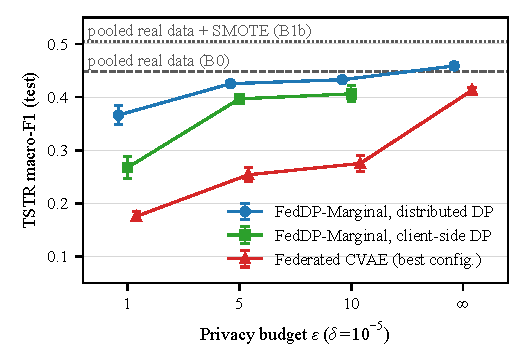
\includegraphics[width=\columnwidth]{graphics/paper/Fig3_python.pdf}
\caption{TSTR macro-F1 (bars: one seed standard deviation) against the privacy budget for FedDP-Marginal with distributed noise (MG) and client-side noise (MGl), and for the best CVAE configuration. The $\varepsilon$ axis is categorical (equal spacing). Dashed lines: RFs trained on pooled real data.}
\label{fig:tstr_eps}
\end{figure}

The cost of DP differs between the routes. Measured against its own non-private release with \eqref{eq:decision_rule}, FedDP-Marginal loses 0.076 (RF) and 0.122 (MLP) at $\varepsilon = 1$, 0.017 and 0.033 at $\varepsilon = 5$, and 0.026 with the MLP at $\varepsilon = 10$, where the RF gains 0.012. For the CVAE route, 11 of 12 such comparisons are worse, with losses of up to 58\% of the synthetic-only macro-F1. Without DP the marginal generator is also better than the CVAE (RF $+0.044$, MLP $+0.046$). Client-side noise costs FedDP-Marginal most at small budgets, because the sum then carries $K$ times the variance.

In fidelity, FedDP-Marginal matches the per-column distributions more closely at $\varepsilon = 5$ and 10 (Wasserstein distance 0.037 and 0.049 against 0.194 and 0.176 for M1); at $\varepsilon = 1$ the two are close (0.194 against 0.235). A classifier still separates synthetic from real rows almost perfectly for every generator, private or not (C2ST AUC 0.9995--1.0000). Utility for an IDS therefore does not mean that the synthetic packets look real.

\subsection{RQ3: What Each Protection Costs and Protects}\label{subsec:rq3}
\textit{Secure aggregation.} For FedDP-Marginal, the release through SecAgg$^+$ (MGs-nodp) sends $1.39\times$ the bytes per round of the same release in plain Flower rounds (MGp-nodp; 0.158 against 0.114\,MB) and takes $1.06\times$ the time of the three rounds (21.6 against 20.4\,s, mostly simulator start-up). Utility is unchanged, because the secure sum equals the exact sum. For the CVAE, SecAgg$^+$ costs $1.12\times$ the time per round and $1.52\times$ the bytes per parameter, and 7 of 8 utility comparisons show no effect. DP-SGD multiplies the time per round by 1.9.

\textit{Empirical leakage.} The attack on the released tables of FedDP-Marginal passes its positive control (AUC 0.835 on noise-free tables of 500 records). Averaged over the three seeds, its AUC is 0.573 without DP and 0.515, 0.525 and 0.539 with DP at $\varepsilon = 1$, 5 and 10; a record bootstrap puts the drops at 0.059 [0.052, 0.065], 0.048 [0.042, 0.055] and 0.034 [0.029, 0.040], all of which pass \eqref{eq:decision_rule}. In absolute terms the leakage is small: at 1\% false positives the attack identifies 1.9\% of the training records without DP and 1.1--1.4\% with DP, against 1\% for a random guess. SecAgg$^+$ alone does not change these numbers, since it hides each gateway's tables, not what their sum reveals. For the CVAE, the attack on synthetic data stays near chance (0.488--0.494) at every $\varepsilon$, including $\infty$, but fails its positive control (0.510), and the model-access attack passes its control (0.647) yet finds no leakage in the federated models (0.497--0.506); there, DP provides the formal guarantee without a measurable reduction.

\textit{Trust and protected unit.} Table~\ref{tab:protection} summarizes the options of FedDP-Marginal at $\varepsilon = 5$. With the noise split over all five gateways, the guarantee degrades to $\varepsilon = 14.2$ if only one gateway is honest; this value grows with the federation (25.4 for 10 and 49.9 for 20 gateways). A threshold $t = 3$ keeps $\varepsilon \le 5$ with any three honest gateways and changes the utility by $-0.005$ to $+0.016$ across budgets. Protecting a whole TCP stream costs 0.03--0.05 macro-F1, because 90\% of the streams contribute a single packet. A whole capture (up to 1,277 packets) can be protected only by bounding its contribution to $m = 25$--100 packets: the guarantee then covers the whole capture, but too little data remain (macro-F1 0.09--0.18). By design, the noise-free sums do not depend on how the rows are spread, nor the total noise on $K$ when $t = K$. Single-seed runs of MGs at $\varepsilon = 5$ agree: $\alpha_{\mathrm{dir}} = 0.1$ and 10 give the identical 0.398, and 10 and 20 gateways give 0.400 and 0.415.

\begin{table}[!t]
\centering
\caption{Protection Options of FedDP-Marginal at $\varepsilon = 5$, With the Non-Private References}
\label{tab:protection}
\scriptsize
\setlength{\tabcolsep}{2.8pt}
\begin{tabular}{l l c c c c}
\toprule
\textbf{Config.} & \textbf{Protection} & \textbf{Macro-F1} & $\boldsymbol{\varepsilon_{h=5}}$ & $\boldsymbol{\varepsilon_{h=1}}$ & \textbf{MIA} \\
\midrule
MGp-nodp       & none                     & 0.459\,$\pm$\,0.007 & $\infty$ & $\infty$ & 0.573 \\
MGs-nodp       & SecAgg$^+$ only          & 0.459\,$\pm$\,0.007 & $\infty$ & $\infty$ & 0.573 \\
MGl-eps5       & client-side DP           & 0.397\,$\pm$\,0.006 & 5.00 & 5.00 & -- \\
MGr-eps5       & distributed DP, $t = 5$  & 0.425\,$\pm$\,0.004 & 5.00 & 14.2 & 0.525 \\
MGr-t3-eps5    & distributed DP, $t = 3$  & 0.420\,$\pm$\,0.009 & 3.72 & 10.1 & 0.524 \\
MGr-t2-eps5    & distributed DP, $t = 2$  & 0.425\,$\pm$\,0.011 & 2.94 & 7.6  & 0.517 \\
MGr-strm1-eps5 & stream unit, $m = 1$     & 0.376\,$\pm$\,0.007 & 5.00 & 14.2 & -- \\
MGr-cap50-eps5 & capture unit, $m = 50$   & 0.177\,$\pm$\,0.020 & 5.00 & 13.0 & -- \\
\bottomrule
\end{tabular}

\vspace{2pt}
\parbox{\columnwidth}{\scriptsize $\varepsilon_{h}$: guarantee when $h$ of the 5 gateways add their noise share; with $t < 5$ the target holds whenever $t$ gateways are honest. MIA: mean calibrated AUC of the attack on the released tables over three seeds (positive control 0.835; --: not attacked).}
\end{table}

\subsection{RQ4: Requirement-Driven Configuration}\label{subsec:rq4}
A single utility ranking does not settle the choice: the best configurations differ more in what they protect and cost than in macro-F1. The recommendation rule therefore proceeds in five steps. It (i) keeps only valid configurations (those whose guarantee covers everything they release); (ii) applies the trust requirement (an untrusted server needs SecAgg$^+$ or client-side DP, and colluding gateways need client-side DP or a threshold $t$); (iii) removes configurations that exceed the limits on $\varepsilon$, bandwidth, rounds or MIA AUC; (iv) keeps the Pareto front over utility, $\varepsilon$, the use of SecAgg$^+$ and cost, where utility within the seed spread, $\varepsilon$ within 2\% and cost within 5\% count as equal; and (v) picks the front member with the highest priority metric (macro-F1 or rare-class recall) and reports those within its seed spread as ties. Here $\varepsilon$ is the guarantee under the scenario's trust assumption: where gateways may collude, it is the value with one honest gateway, so consortium takes MGr-t2-eps5 (7.63) over client-side noise; where gateways are trusted, a threshold configuration counts with its target, so MGs-t3-eps5 counts as $\varepsilon = 5$, not 3.72. Table~\ref{tab:recommend} lists the outcome for eleven deployment scenarios.

\begin{table}[!t]
\centering
\caption{Recommended Configuration per Deployment Requirement}
\label{tab:recommend}
\scriptsize
\setlength{\tabcolsep}{2.5pt}
\begin{tabularx}{\columnwidth}{l >{\raggedright\arraybackslash}X l c c}
\toprule
\textbf{Scenario} & \textbf{Requirement} & \textbf{Choice} & \textbf{F1} & $\boldsymbol{\varepsilon}$ \\
\midrule
lab              & all parties trusted, no DP           & MGp-nodp       & 0.459 & $\infty$ \\
hidden-tables    & untrusted server, no DP              & MGs-nodp       & 0.459 & $\infty$ \\
cloud-aggregator & untrusted server, $\varepsilon \le 5$ & MGd-eps5      & 0.426 & 5 \\
rare-attacks     & as above, rare recall first          & MGd-eps5       & 0.426 & 5 \\
strict-privacy   & untrusted server, $\varepsilon \le 1$ & MGs-t3-eps1   & 0.373 & 1 \\
low-bandwidth    & $\varepsilon \le 10$, $\le 100$\,MB total & MGs-t3-eps10 & 0.449 & 10 \\
consortium       & gateways may collude, $\varepsilon \le 10$ & MGr-t2-eps5 & 0.425 & 7.63 \\
honest-majority  & $\ge 3$ honest, $\varepsilon \le 10$, MIA $< 0.55$ & MGs-t3-eps10 & 0.449 & 10 \\
gateway-dropout  & $\ge 3$ honest, $\varepsilon \le 5$  & MGr-t2-eps5    & 0.425 & 3.94 \\
session-privacy  & TCP-stream unit, $\varepsilon \le 5$ & MGs-strm1-eps5 & 0.397 & 5 \\
capture-privacy  & capture unit, $\varepsilon \le 10$  & MGr-cap50-eps5$^\dagger$ & 0.177 & 5 \\
\bottomrule
\end{tabularx}

\vspace{2pt}
\parbox{\columnwidth}{\scriptsize F1: TSTR macro-F1; $\varepsilon$: the guarantee that holds under the scenario's trust assumption. $^\dagger$Holds formally by using at most 50 packets of each capture; not practical at this utility.}
\end{table}

Fig.~\ref{fig:pareto} places every valid configuration by utility and total traffic: all FedDP-Marginal variants stay below 1.4\,MB per run, at least six times less than any CVAE route (8.4--191\,MB), and make up 17 of the 18 configurations on the Pareto front. Two choices come with ties: lab ties MGp-nodp with MGs-nodp, the same tables sent through SecAgg$^+$ (0.158 instead of 0.114\,MB per round), and cloud-aggregator ties MGd-eps5, whose secure sum is simulated in-process, with MGs-t3-eps5 (0.420), which runs through Flower's SecAgg$^+$.

\begin{figure}[!t]
\centering
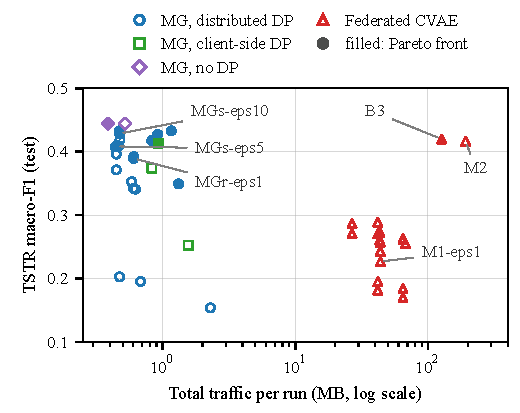
\includegraphics[width=\columnwidth]{graphics/paper/Fig4_python.pdf}
\caption{TSTR macro-F1 against total traffic per run (log scale) for all valid configurations. MG: FedDP-Marginal, including its Gaussian ablation (MGd, summed in-process) and second-order ablation (MGb); MGp: plain Flower sum without SecAgg$^+$. The traffic of the client-side variants (MGl) is estimated, as in Table~\ref{tab:main}. Filled markers: Pareto front over utility, $\varepsilon$ and cost.}
\label{fig:pareto}
\end{figure}

\subsection{Discussion and Limitations}\label{subsec:limitations}
\textit{Why the marginal route degrades less under DP.} FedDP-Marginal spends its budget on three releases, each a single sum with a known sensitivity, so the noise is added once per cell. Its pooled pairwise release keeps the per-cell signal high. Because each release is a sum, distributed noise and secure aggregation fit it exactly. In the DP-SGD setup used here, noise is added at every local step and cannot be shared across gateways (Section~\ref{subsec:accounting}). In return, the marginal route captures only pairwise dependencies through one tree, and second-order structures did not help on this data.

\textit{Limitations.}
\begin{itemize}
    \item The study uses one dataset at the packet level, and generated packets have no stream context. The normal traffic was exported from PCAP files with the authors' settings; one attack capture was published with both directions, so 18.1\% of the \texttt{SYN} training rows are packets sent by the broker.
    \item $\varepsilon$ protects one packet by default. One capture group contributes up to 188 packets of a rare class, so the group bound for a whole capture is vacuous. Labels, class counts, preprocessing statistics and validation-based tuning lie outside $\varepsilon$.
    \item The standardization statistics, the skewness test, the clipping range and the category lists are fitted on the pooled training split. A deployment would need fixed public ranges, a secure protocol, or a DP release of these statistics before Release~1, which would consume part of the budget.
    \item The study assumes honest-but-curious parties, and the federation, including SecAgg$^+$, is simulated on one machine, so no real network or device costs are measured.
    \item Three seeds give a rough spread, and the verdicts hold for this test split. A CVAE with distributed noise, FLAIM or AIM themselves, and other deep generators were not compared; the detector with shared noise used Gaussian accounting and a small grid tuned on one seed.
\end{itemize}

\section{Conclusion}\label{sec:conclusion}
PP-FedData generates synthetic IoT-MQTT traffic across gateways that cannot share raw packets; this paper compared two federated generators under the same partitions, privacy budgets and secure aggregation. FedDP-Marginal, which releases three sums of noisy count tables with Skellam noise split across gateways and summed by SecAgg$^+$, kept 0.366--0.433 test macro-F1 at $\varepsilon = 1$--10, against 0.176--0.275 for a federated CVAE trained with DP-SGD, while sending less than 1\,MB per run. With the noise added at each gateway, the CVAE's own trust model, it still led at every budget. Secure aggregation cost little and no utility. DP cost FedDP-Marginal up to 0.12 macro-F1 at $\varepsilon = 1$ and at most 0.03 at $\varepsilon = 5$ and 10, and lowered the AUC of an attack on its released tables from 0.573 to 0.515--0.539, although the leakage was small in both cases. Synthetic data did not improve an IDS whose real data could be pooled, synthetic packets remained distinguishable from real ones, and the guarantee is per packet unless a stream-level unit is chosen. The framework is therefore a way to train or complete an IDS where traffic must stay local, and its requirement-driven rule tells a deployment which protection to choose and what it will cost.

Future work will evaluate other IoT datasets, compare against FLAIM, AIM and a CVAE with distributed noise, estimate the preprocessing statistics and select hyperparameters privately, and measure the protocols on physical gateways over a real network.

\section*{Acknowledgment}
This research was conducted within the Capstone Project Program of the Faculty of Information Assurance, FPT University, Hanoi Campus.

\bibliographystyle{IEEEtran}
\bibliography{references/reference}

\end{document}